
\chapter{Effect of second order piezoelectricity on electric dipole in strain-tuned InGaAs/GaAs quantum dots}\label{chap:2order_piezo}

Semiconductor QDs provide due to zero-dimensional confinement extremely sensitive electronic structure to tiny variations of their shape, size, composition, and built-in strain fields. %Moreover, their electronic and optical properties can be reversibly tuned by external fields: electric~\cite{Gerardot_2007, Vogel_2007} and magnetic~\cite{Stevenson_2006} or strain~\citep{kleDresden}. This tunability of properties makes QDs suitable candidates to create single-photon sources for optical fibre communication~\cite{Huffaker1998} or produce entangled photon pairs~\cite{Trotta:16}
%
%
Moreover, their electronic and optical properties can be post-processionally tuned by external fields: electric~\cite{Gerardot_2007, Vogel_2007} and magnetic~\cite{Stevenson_2006} or strain~\citep{kleDresden}. This tunability of properties makes QDs suitable candidates to create single-photon sources for optical fibre communication~\cite{Huffaker1998} or produce entangled photon pairs~\cite{Trotta:16}.

Bester et. al~\citep{Bester:06, Bester:06_2} firstly mentioned about the importance of nonlinear terms in the expansion of electrical polarization $\mathbf{P}$ as a function of strain $\eta$ in III--V semiconductor. They found that for large $\eta$, which is usually present in self-assembled QDs obtained by the Stranski-Krastanov growth~\cite{Grundmann}, the second order term might dominate compare to the first ones.

In Ref.~\cite{Aberl:17} it has been recently shown that the vertical electron-hole dipole moment $p$ in InGaAs/GaAs QDs can be tuned by externally-applied, anisotropic in-plane stress~\cite{Trotta:12,Trotta:13} and even its inversion can be achieved. Furthermore, it was found that the pronounced tuning of $p$ can only be described by nonlinear terms in the expansion of the piezoelectric tensor. 

In this chapter, we provide more details about the effects of the second-order piezoelectric terms on the tunability of $p$ in strain-tuned InGaAs QDs. Moreover, we discuses other potentialities such as effects of size, In contribution, or a pre-stress causing by bonding onto a piezo acuatoator to tune emission energy and $p$. 

%The importance of a nonlinear piezoelectric terms in expansion of effect was firstly mentioned by Cibert et al.~\cite{Cibert_PRB1996_Nonlinear_piezoII_VI,cibert_JCG_1992_CdTe_piezo}
\label{sec:2order_piezo}

%ts including cryogenic temperatures and magnetic fields. The exploitation of the quantum nature of light has triggered an intensive research activity in the field of quantum computation and telecommunications. One major issue that an ideal source of non-classical light should fulfilled is the emission of single photons at a time. Besides single photon emitters like single molecules [30] or nitrogen vacancy centers in diamond [31], self-assembled quantum dots (QDs) embedded in a semiconductor matrix have emerged as promising candidates for solid-state applications [32] since they can be electrically addressed upon their deterministic integration in p–i–n diode and/or photonic nanomembrane structures [18]. However, unavoidable structural asymmetries arising from compositional fluctuations in the confining potential barriers for the carriers in the QDs and their shape, as well as the stochastic process in QDs formation, lead to fluctuations in their optical properties which humpers their applicability for advanced quantum optics. Hence, post-processing through the application of external perturbations, i.e. magnetic, electric and/or strain fields, to compensate the inherent asymmetries in self-assembled QDs are mandatory [19, 33, 34]


%Contrary to the case of nanowire waveguides that allow broadband wavelength operation, in optical micro-cavity structures there are two stringent requirements for an efficient light extraction: spectral and spatial matching of the QD with the cavity mode. The latter can be performed deterministically by in situ lithography or QD location followed by lithography after growth [96–99]. In these approaches, the position of the QD is known before the fabrication of the cavity structure. 
%Other approaches based on the definition of the QD nucleation sites by ex situ lithography/patterning techniques with nanometer resolution [100, 101], followed by regrowth procedures have also been reported [101]. The spectral tuning of the QD emission with the cavity modes is conventionally realized reversibly by applying magnetic fields [102], electric fields [103] or varying the temperature [104]. However, electric fields lead to PL quenching due to an increased electron and hole wavefunctions separation [105] and temperature tuning is detrimental for the emission efficiency and induce dephasing due to the interaction of the excitons with phonons. Strain-tuning to frequency-match the QD photons with the cavities modes by employing piezoelectric actuators has been demonstrated as a suitable strategy to overcome these problems in an elegant manner. The key ingredient is related to the fact that the QD and the cavity mode shift at a different rate when stress is applied.



%\begin{figure}
%	\centering
%	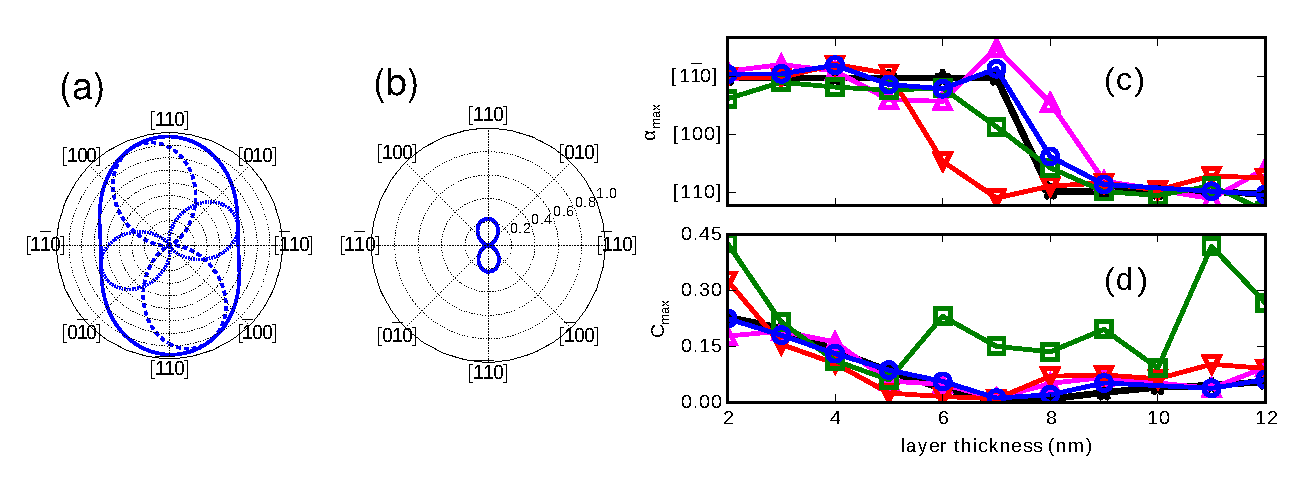
\includegraphics[width=1\linewidth]{/Sci_rep/test/a}
%	\caption{test}
%	\label{fig:kt_sectext}
%\end{figure}

\newpage 





\section{Expansion of electrical polarization $\mathbf{P}$ into strain terms}

The Taylor expansion of ${\bf P}$ in terms of $\eta$ is obtained as
%
\begin{equation}
\label{eq:2ndPiezGeneral}
P_{\mu}=\sum_je_{\mu j}\eta_j+\frac{1}{2}\sum_{jk}B_{\mu jk}\eta_j\eta_k+\dots,
\end{equation}
%
where $e_{\mu j}$ is the linear and $B_{\mu jk}$ are the quadratic piezoelectric coefficients. In $\mathrm{III-V}$ zinc blende semiconductors most of $e$ and $B$ terms are equal to each other, only one linear ($e_{14}$) and three non-linear ($B_{114}$, $B_{124}$, $B_{156}$) terms remain independent in Eq.~(\ref{eq:2ndPiezGeneral}) up to the second order~\cite{Beya-Wakata2011}. It is then convenient to rewrite Eq.~(\ref{eq:2ndPiezGeneral}) as ${\bf P}={\bf P}_{l}+{\bf P}_{nl}$, where ${\bf P}_{l}$ is the linear term
%
%
\begin{equation}
\label{eq:1stPiez}
{\bf P}_{l}=e_{14}\begin{pmatrix}\eta_4\\\eta_5\\\eta_6\end{pmatrix},
\end{equation}
%
and ${\bf P}_{nl}$ the nonlinear one:
%
\begin{equation}
\label{eq:2ndPiez}
{\bf P}_{nl}=B_{114}\begin{pmatrix}\eta_1\eta_4\\\eta_2\eta_5\\\eta_3\eta_6\end{pmatrix}+
B_{124}\begin{pmatrix}\eta_4(\eta_2+\eta_3)\\\eta_5(\eta_3+\eta_1)\\\eta_6(\eta_1+\eta_2)\end{pmatrix}+
B_{156}\begin{pmatrix}\eta_5\eta_6\\\eta_4\eta_6\\\eta_4\eta_5\end{pmatrix}.
\end{equation}
%
%
Here $\eta$-s are indexed according to the Voigt notation,~i.e.,~ $\eta_1=\eta_{xx}$, $\eta_2=\eta_{yy}$, $\eta_3=\eta_{zz}$, $\eta_4=2\eta_{yz}$, $\eta_5=2\eta_{xz}$, $\eta_6=2\eta_{xy}$~\cite{Beya-Wakata2011} where $x,y,z$ denote the crystallographic axes of the conventional cubic unit cell of the zinc blende lattice.
%
%$1=xx,2=yy,3=zz,4=yz,5=xz,6=xy$~\cite{Beya-Wakata2011}.
%
Note that even though the coefficients of the expansion into cubic
%higher order 
terms was provided by Tse and colleagues~\cite{Tse2013}, we restrict ourselves to second-order ones in this work and show that for the small externally applied strain magnitude of only 0.1~\%~\cite{Aberl:17} we can describe experimental results obtained by Aberl~\cite{Aberl:17} accurately within this restriction. 


\section{Single-particle calculations based on 8-band $\bf{k \cdot p}$ method}




Before we present the results of full electronic structure calculations for the InGaAs QDs obtained by the nextnano$^3$ simulation suite~\cite{Birner:07}, we analyze the additional piezoelectric polarization established by the externally applied stress. In particular, we show that despite the small strains established in the InGaAs layer as a consequence of deformation of a piezo actuator the sample is bonded on, the established piezo-polarisation is dominated by the second order piezo-constants $B_{\mu,j,k}$. For simplicity, in this section we tread the InGaAs QD as two-dimensional layer with tetragonal symmetry.    


For comparison, we have used the envelope function approximation based on 8-band ${\bf k}\cdot{\bf p}$ perturbation method using the nextnano$^3$ simulation suite~\cite{Birner:07}. These simulations can be divided into 4~following~steps:
\begin{itemize}
	\item [1.] definition of the simulation structure (shape, material parameters),
	\item[2.] calculations of the strain in the structure by minimization of the elastic energy,
	\item[3.] calculations of the electric field in the structure using the Poisson equation and calculation of the piezoelectric field,
	\item[4.] solving the single-electron Schrödinger equation using envelope function approximation.
\end{itemize}
%
%We have calculated the electronic structure of InGaAs/GaAs QDs with the shape of truncated cones as shown in Fig.~\ref{fig:2order:QDStruct} using the envelope function approximation based on 8-band ${\bf k}\cdot{\bf p}$ perturbation method using the nextnano$^3$ simulation suite~\cite{Birner:07}. 
The calculations include full treatment of the elastic strain field employing the Bir-Pikus hamiltonian~\cite{BirPik}. Piezoelectric fields up to the second order in the strain are included self-consistently. Material parameters used in our simulations are listed in Appendix~\ref{app:material_params}. 





We have simulated two structures of InGaAs/GaAs QDs with the shape of truncated cones that we call QD$_1$ and QD$_2$ differing in size and In alloy distribution.
%
\begin{figure}[!ht]
	\renewcommand{\tabcolsep}{2pt}
	\begin{center}
		\begin{tabular}{c}
			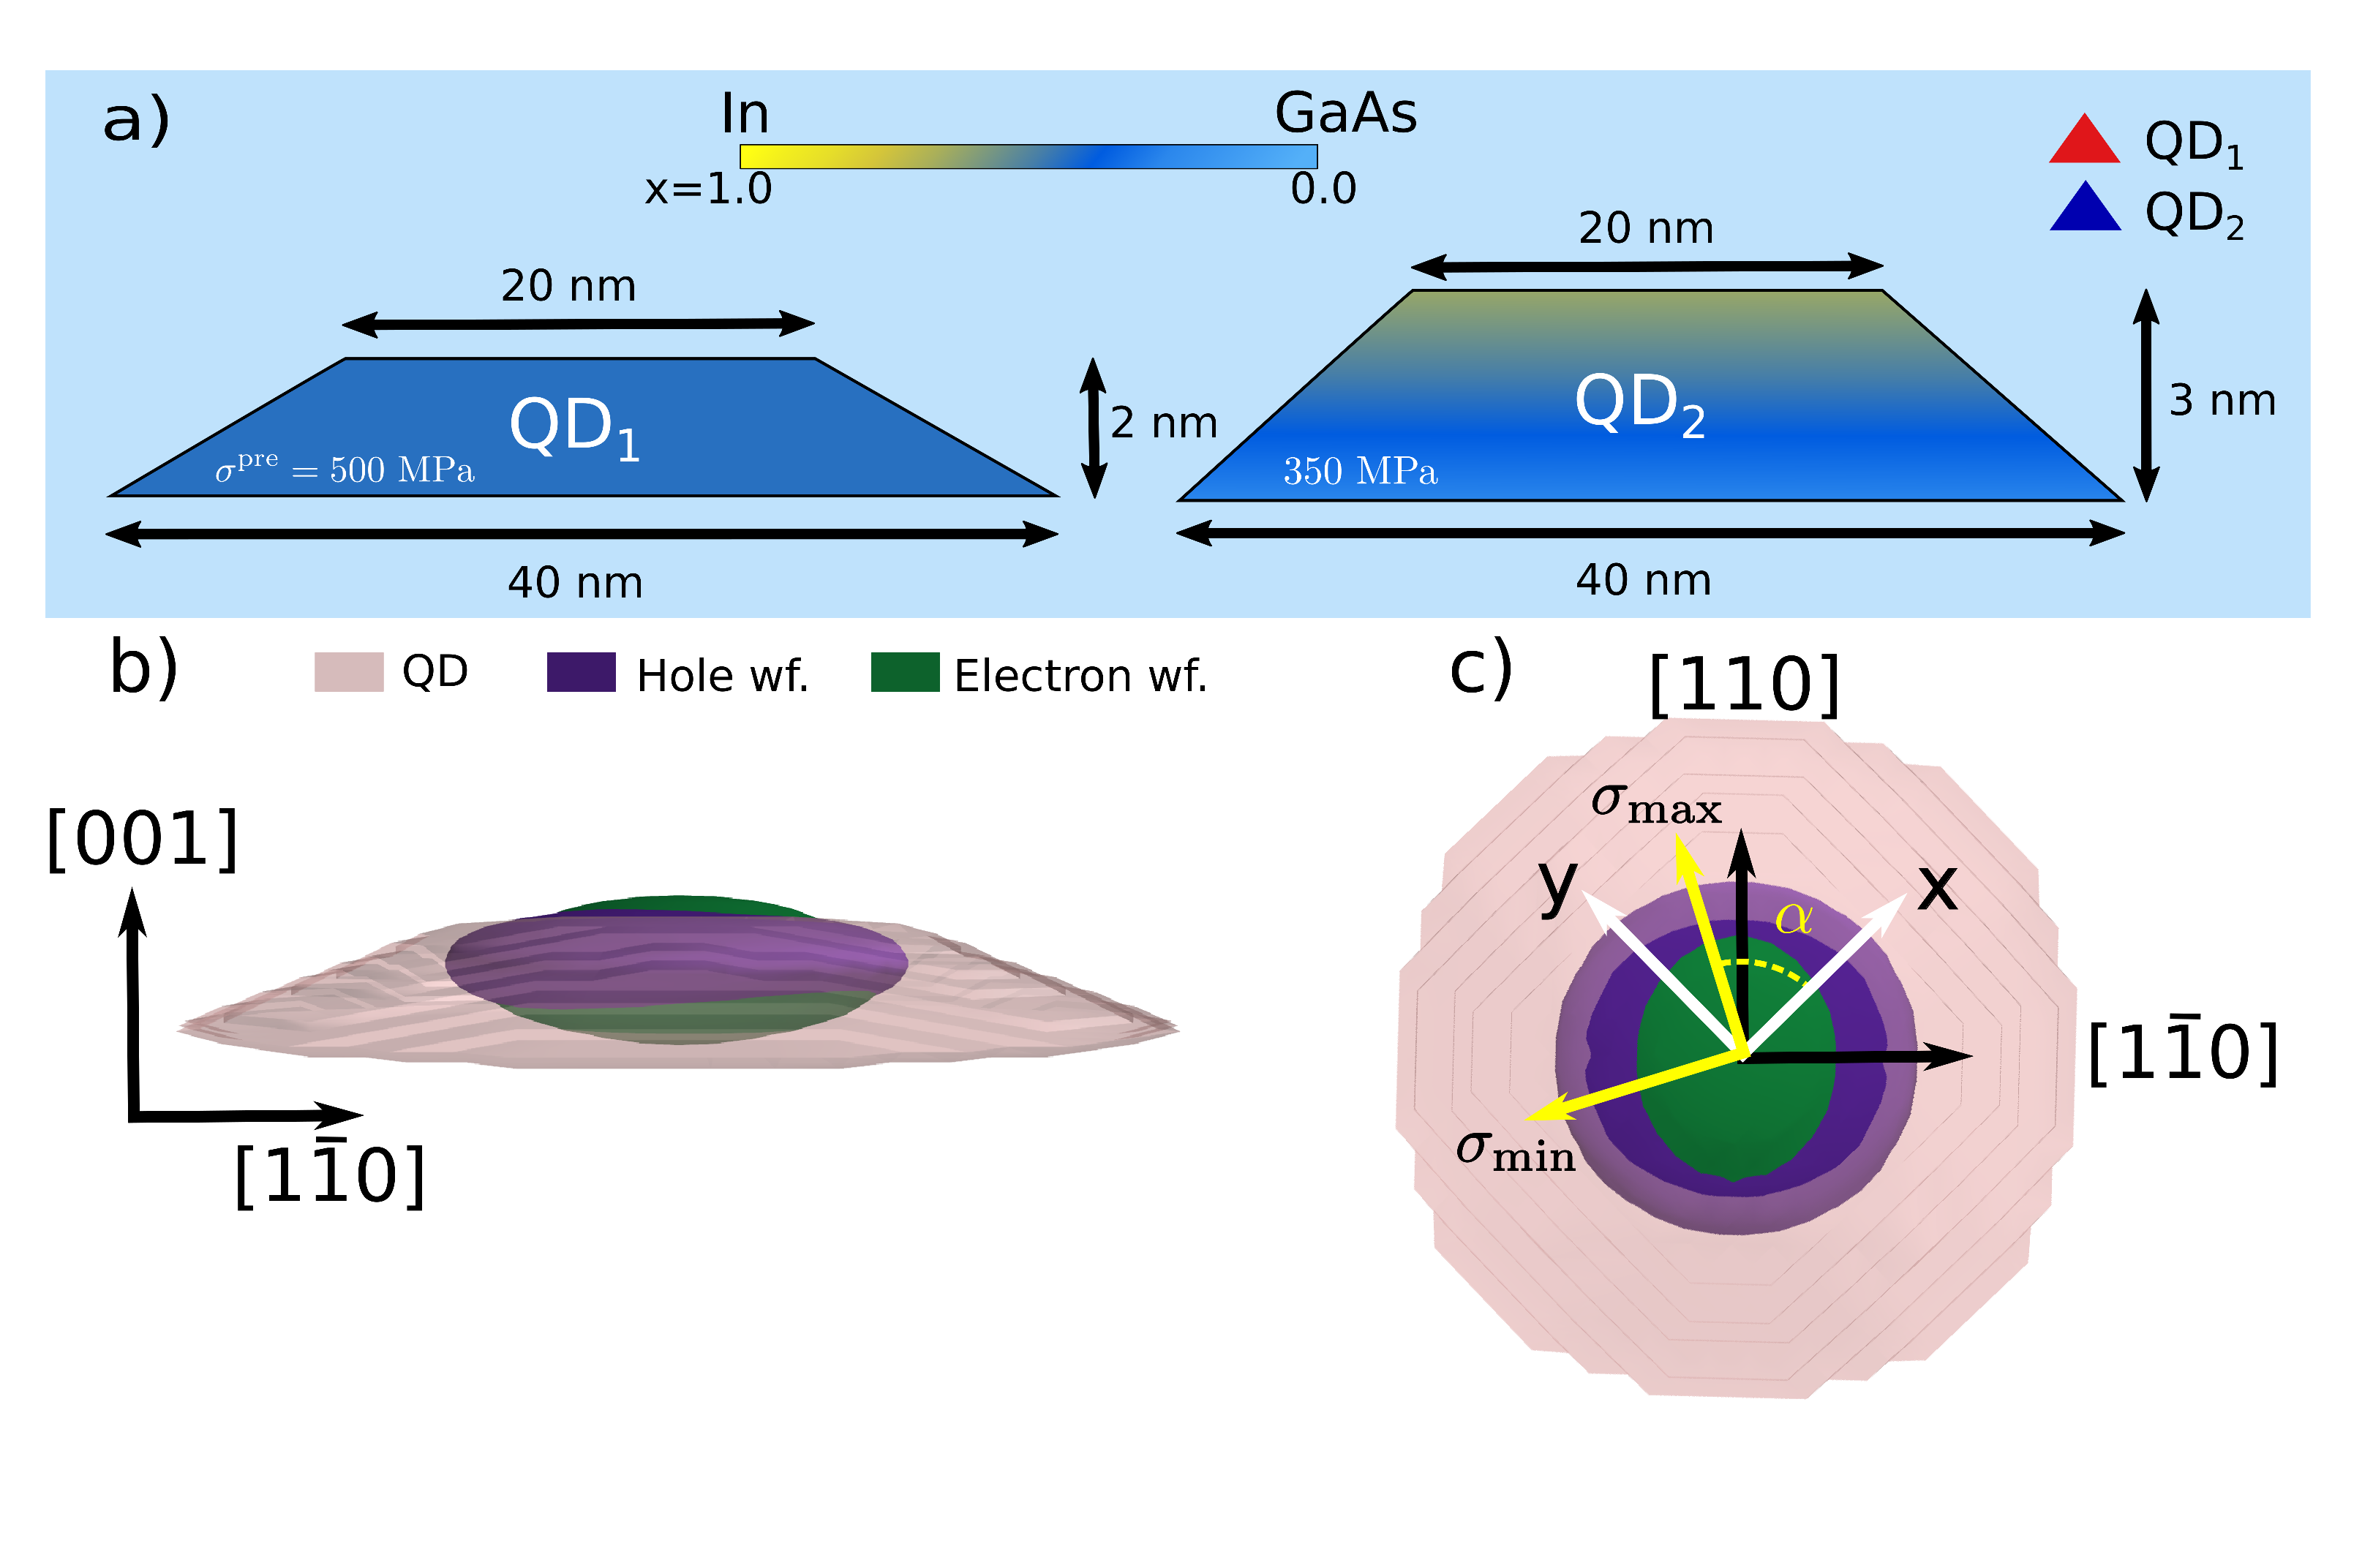
\includegraphics[width=0.8\textwidth]{2_order/180204_structura_wo-gradient_w_triangles_and_wfuncions_vs5} \\ 
		\end{tabular}
	\end{center}
	\caption{In panel a) we show the side view of the calculated In$_{{x}}$Ga$_{1-x}$As/GaAs QD$_1$ and QD$_2$ structures. Both of the QDs have the shape of truncated cones with base and top diameters of 40~nm and 20~nm, respectively, the height is 2~nm~(3~nm), In composition is constant of 0.45 (linearly increasing from 0.25 at the bottom to 0.65 at the apex), and $\sigma^\text{pre}=500$~MPa ($\sigma^\text{pre}=350$~MPa) for QD$_1$ (QD$_2$). Panels b) and c) show the top and side view, respectively, of the typical simulated dot (grey), and calculated electron (green) and hole (blue) probability densities. The wavefunctions are given as isosurfaces encircling 70\% of the probability.
		\label{fig:2order:QDStruct}}
\end{figure}

Side views of QD$_1$ and QD$_2$ are shown in Fig.~\ref{fig:2order:QDStruct}~a) and their parameters were deliberately chosen so that the calculated dependencies of the emission energy $E_0$ and of the dipole moment $p$ on the hydrostatic part of the applied anisotropic stress $\sigma_{\mathrm{max}}+\sigma_{\mathrm{min}}$ match the experimental results taken from Ref.~\cite{Aberl:17}, see Fig.~\ref{fig:TheorVsExp}. The variables $\sigma_{\mathrm{max}}$ and $\sigma_{\mathrm{min}}$ denote the principal stresses~\cite{Trotta:15} applied externally by the two-dimensional piezo actuator. In  Ref.~\citep{Aberl:17} it was shown that $\sigma_{\mathrm{max}}$ was applied at an angle of $\alpha=55^{\circ}$ with respect to the crystal axis [100], resulting in the principal axis system of the externally applied stress as shown in Fig. \ref{fig:2order:QDStruct}. The various coordinate systems used in our model as well as the single-particle wavefunctions of electrons and holes are indicated in Fig. \ref{fig:2order:QDStruct} b) and c). The connection between the Cartesian and the principal stresses is derived in~Appendix~\ref{app:principal_stress}.

As discussed in Ref.~\cite{Aberl:17}, in course of bonding the sample onto the piezo actuator, a shear prestess $\hat\sigma^\text{pre}$ independent on the voltage applied to the piezo is exerted on the sample. Consequently, in order to match the measured values of $p$ with results of our calculations we needed to allow for different magnitude of $\sigma^\text{pre}$ of 500 and 350~MPa that acted on QD$_1$ and QD$_2$, respectively.

Experimentally acquired dependencies of $p/e$ on $\sigma_{\mathrm{max}}+\sigma_{\mathrm{min}}$ follow a linear behaviour, therefore, we have fitted the (gray) data by linear model derived by Klenovský et al.~\cite{Klenovsky_2018_InGaAs_straintuned}
\begin{eqnarray}
p/e\approx A^{\mathrm{QD}}\left(\sigma_\mathrm{max}+\sigma_\mathrm{min}\right)+b, \label{eq:strain_model}
\end{eqnarray}
which allow us to describe the evolution of $p/e$. Results of the fit by model~(\ref{eq:strain_model}) are listed in Tab.~\ref{tab:exp_slopes} in Appendix~\ref{app:slopes_of_dipole}.

%


\begin{figure}[!ht]
	\centering
	\renewcommand{\tabcolsep}{2pt}
	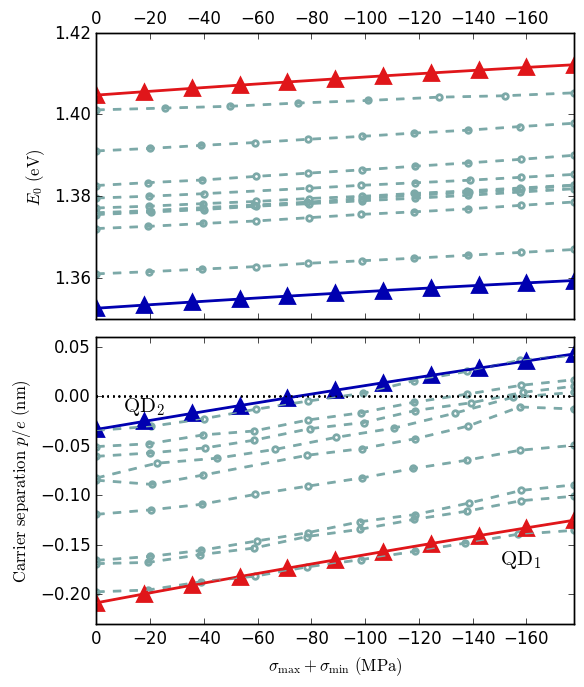
\includegraphics[width=0.5\textwidth]{/2_order/Energy/2018-02-04__171219_8x8_neotocena_35deg_pres500___theoryVSexperiment} 
	\caption{
		Dependencies of $E_0$ (top panel) and $p/e$ (bottom panel) on $\sigma_{\mathrm{max}}+\sigma_{\mathrm{min}}$ experimentally obtained from $\mu$PL measurements of nine InGaAs QDs~\cite{Aberl:17} (dashed curves) and that calculated for QD$_1$ (full red curve) and QD$_2$ (full blue curve). The letter $e$ denotes the elementary charge.}
	%
	%two different QDs, i.e. first with base and top diameter of 30~nm and 15~nm, respectively and height of 3~nm. 
	\label{fig:TheorVsExp}
\end{figure}

\section{Effect of second order of piezoelectricity}
%
\begin{figure}[h]
	%\renewcommand{\tabcolsep}{2pt}
	\begin{center}
		\begin{tabular}{cc}
			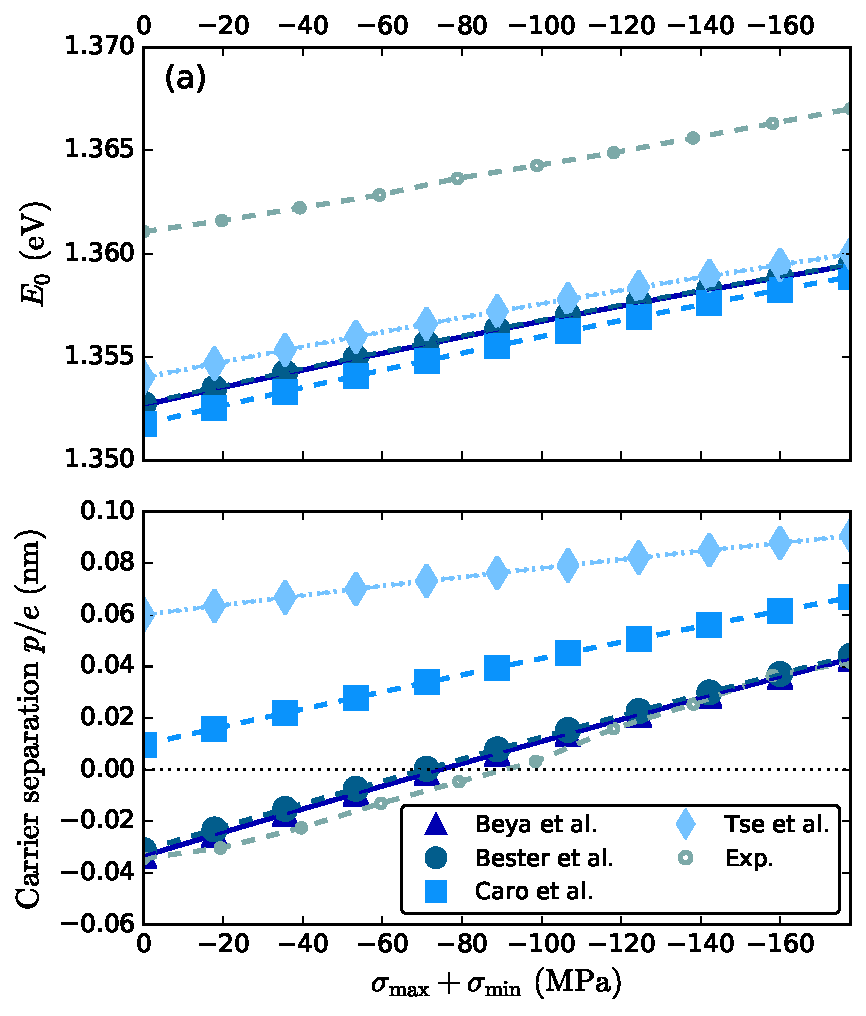
\includegraphics[width=0.5\textwidth]{/2_order/Energy/FINAL_a__171219_8x8_neotocena_++_nn+_35deg_pres350___40x20x3-25-65_350_piezo2ndorder} & 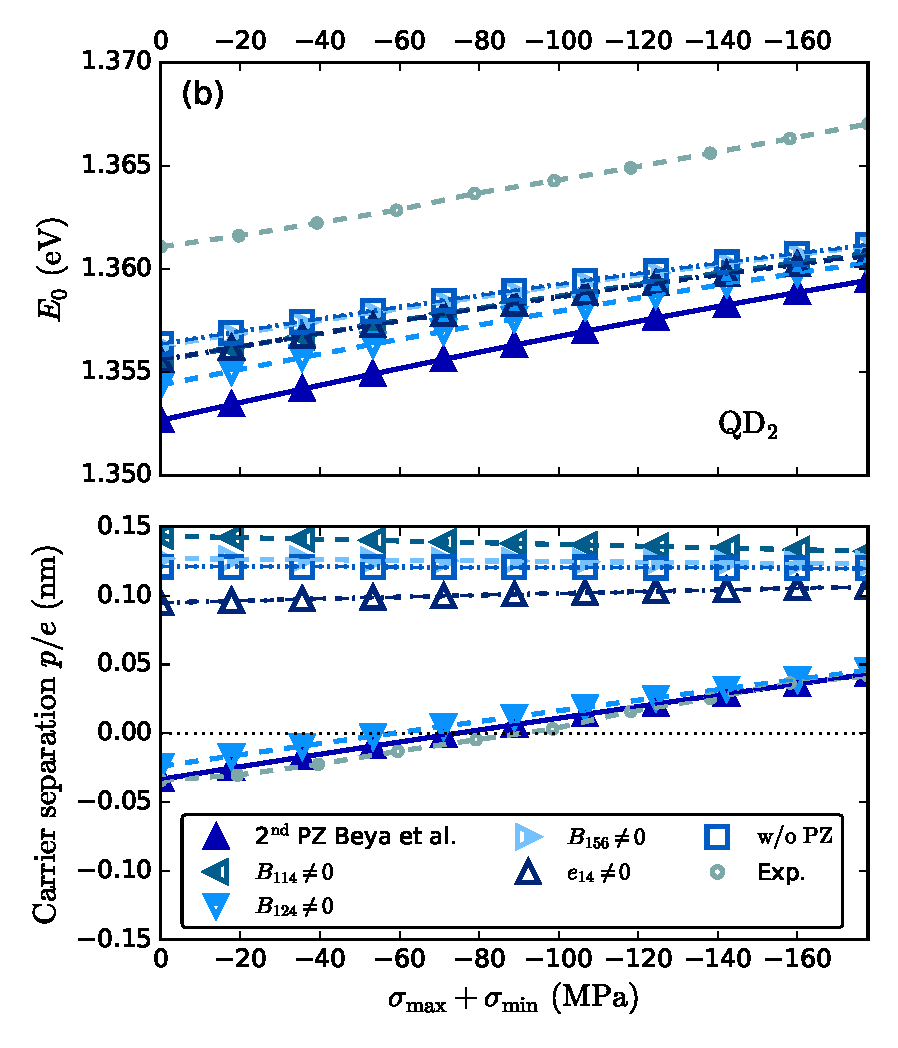
\includegraphics[width=0.5\textwidth]{/2_order/Energy/FINAL_b__171219_8x8_neotocena_++_nn+_35deg_pres350___40x20x3d0_piezo2ndorder_jednotlive_cleny}\\
		\end{tabular}
	\end{center}
	\caption{
		(a) Comparison of calculation results based on four published sets of parameters of second order piezoelectric coefficients, i.~e., Refs.~\cite{Beya-Wakata2011,Bester:06,Caro2015,Tse2013} for QD$_2$. (b) Comparison of dependencies of $E_0$ and $p/e$ on $\sigma_{\mathrm{max}}+\sigma_{\mathrm{min}}$ for all piezoelectric parameters equal to zero except of $e_{14}$, $B_{114}$, $B_{124}$, and $B_{156}$ sequentially retaining their values for QD$_2$. In the top panels are presented the dependences of emission energy $E_0$ on applied stress $\sigma_{\mathrm{max}}+\sigma_{\mathrm{min}}$ and that for $p/e$ in lower panels. 
		The experimental data from Ref.~\cite{Aberl:17} are shown by the grey dashed curves in all panels. 
		\label{fig:DiffPiezo}}
\end{figure}

In Ref.~\cite{Aberl:17} it was mentioned that experimental obtained $p/e$ on $\sigma_{\mathrm{max}}+\sigma_{\mathrm{min}}$ can be explained only by including the second-order contribution to the piezoelectric field.
%
Motivated by that, we proceed with the analysis of the evolution of $p/e$ on $\sigma_{\mathrm{max}}+\sigma_{\mathrm{min}}$ for all published second-order piezoelectric parameters listed in Tab.~\ref{tab:second_piezo}. 
%
%
\begin{table*}[!ht]
	\begin{center}
		\caption{Values for the linear and quadratic piezoelectric coefficients $e_{14}$, $B_{114}$, $B_{124}$ and $B_{156}$. The references from which the parameters were taken are identified in the first column. The units of presented piezoelectric constants are $C/m^2$. For In$_x$Ga$_{1-x}$As, the constants were obtained by linear interpolation. \label{tab:second_piezo} 
		}
		\begin{tabular}{c|ccccc}
			\hline \hline
			%Ref. & compound & $e_{14}$ $(C/m^2)$& $B_{114}$ $(C/m^2)$ & $B_{124}$ $(C/m^2)$&$B_{156}$ $(C/m^2)$\\
			Ref. & compound & $e_{14}$ & $B_{114}$  & $B_{124}$ &$B_{156}$\\
			\hline
			\multirow{2}{*}{Beya-Wakata et al.~\cite{Beya-Wakata2011}} & GaAs & $-0.238$ & $-0.4$  & $-3.8$& $-0.7$\\
			& InAs& $-0.115$ & $-0.6$  & $-4.1$& $0.2$\\
			% 
			\hline
			\multirow{2}{*}{Bester et al.~\cite{Bester:06} }& GaAs & $-0.23$ & $-0.439$  & $-3.765$& $-0.492$\\
			& InAs& $-0.115$ & $-0.531$  & $-4.076$& $-0.12$\\
			%
			\hline
			\multirow{2}{*}{Caro et al.~\cite{Caro2015}} & GaAs & $-0.205$ & $-0.99$  & $-3.21$& $-1.28$\\
			& InAs& $-0.111$ & $-1.17$  & $-4.31$& $-0.46$\\
			%		
			\hline
			\multirow{2}{*}{Tse et al.~\cite{Tse2013}} & GaAs & $-0.16$ & $-0.666$  & $-1.646$& $-$\\
			& InAs& $-0.045$ & $-0.653$  & $-1.617$& $-$\\
			\hline \hline
		\end{tabular}
	\end{center}
\end{table*}
%
%
The results for QD$_2$ are shown in Fig.~\ref{fig:DiffPiezo}~(a) and demonstrate that both the inversion of $p$ with $\sigma_{\mathrm{max}}+\sigma_{\mathrm{min}}$ as well as the slopes $A^{\mathrm{QD}}$ and $\partial E_0/\partial(\sigma_{\mathrm{max}}+\sigma_{\mathrm{min}})$ remain remarkably similar among various parameter sets in the literature even though the coefficients differ considerably among them.
For example, the parameter $B_{156}$ has even a different sign between Refs.~\cite{Bester:06} and~\cite{Beya-Wakata2011} or is omitted in Ref.~\cite{Tse2013}.
%


%
%\begin{figure}
%	\begin{center}
	%	\includegraphics[width=0.42\textwidth]{/2_order/FINAL__171219_8x8_neotocena_++_nn+_35deg_pres350___40x20x3d0_piezo2ndorder_jednotlive_cleny}
	%\end{center}
	%\caption{
	%	Comparison of dependencies of $E_0$ and $p/e$ on $\sigma_{\mathrm{max}}+\sigma_{\mathrm{min}}$ for all piezoelectric parameters equal to zero except of $e_{14}$, $B_{114}$, $B_{124}$, and $B_{156}$ sequentially retaining their values for QD$_2$. For comparison, one set of the experimental data from Ref.~\cite{Aberl:17} is given by the grey dashed curve. Otherwise the outline of the figure is the same as that in Fig.~\ref{fig:DiffPiezo}.
	%	\label{fig:DiffPiezoCoeff}}
%\end{figure}


%%
%tady jsem zkoncil
%%%% 

To investigate the origin of that apparent similarity we have performed calculations, in which we have set all piezoelectric parameters equal to zero except of $e_{14}$, $B_{114}$, $B_{124}$, and $B_{156}$ sequentially retaining their values, see Fig.~\ref{fig:DiffPiezo}~(b) for results for QD$_2$. 


Firstly, we note that the dependencies for $E_0$ are very similar irrespective of which piezoelectric parameter is not set to zero. This is connected with the fact that the change of the emission energy from QDs with stress is dominated by its hydrostatic components.

Secondly, the most important piezoelectric parameter is noticeably $B_{124}$. Evidently, the second term in Eq.~(\ref{eq:2ndPiez}) dominates the dependencies of $E_0$ and $p/e$ on $\sigma_{\mathrm{max}}+\sigma_{\mathrm{min}}$. This is not surprising since the magnitude of $B_{124}$ is several times larger than that of $e_{14}$, $B_{114}$, or $B_{156}$~\cite{Beya-Wakata2011}. 


\section{Effect of indium distribution}

\begin{figure}[!ht]
	\renewcommand{\tabcolsep}{2pt}
	\begin{center}
		\begin{tabular}{c}
			%\includegraphics[width=0.4\textwidth]{2017-12-15__170921_35deg_pres200___30x15x3_concentration.eps} \\
			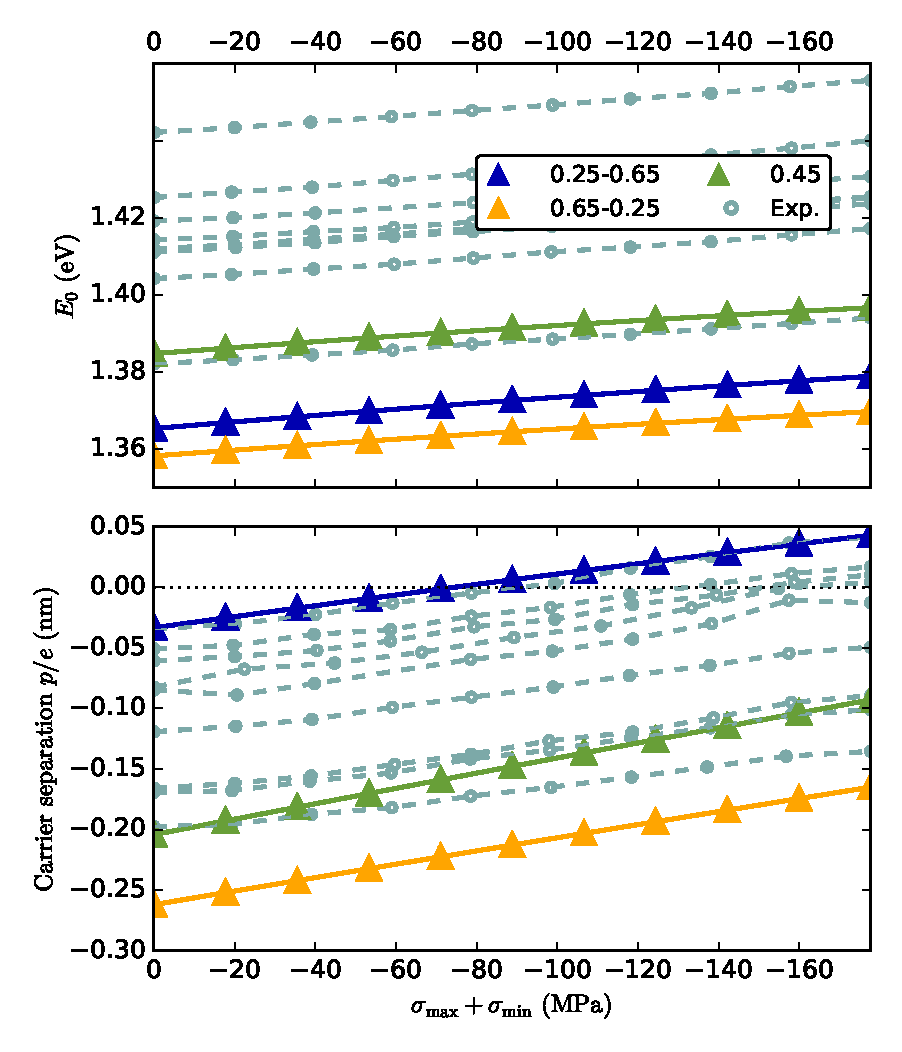
\includegraphics[width=0.5\textwidth]{/2_order/Energy/FINAL__171219_8x8_neotocena_++_nn+_35deg_pres350___40x20x3_concentration} \\
		\end{tabular}
	\end{center}
	\caption{
		Dependencies of $E_0$ (top panel) and $p/e$ (bottom panel) on $\sigma_{\mathrm{max}}+\sigma_{\mathrm{min}}$ experimentally obtained from $\mu$PL measurements of nine InGaAs QDs~\cite{Aberl:17} (dashed curves) and that calculated for different In contents inside QD. The data for In content linearly varying as a function of vertical dimension from 0.25~(0.65) at QD base to 0.65~(0.25) at QD apex are shown as blue~(orange) curves. Those for constant In content of 0.45 are given as green curves. The data calculated assuming second-(first-)order piezoelectricity taken from Ref.~\citep{Beya-Wakata2011} are given as full (open) triangles. All other properties of the dots we the same as for QD$_2$. The letter $e$ denotes the elementary charge.
		\label{fig:TuningByConc}}
\end{figure}
%

Motivated by Refs.~\cite{Grundmann, Fry:00} discussing the influence of indium distribution inside InAs/GaAs QDs on $p$ we have also studied the effect of that in our stress-tuned dots. In Fig.~\ref{fig:TuningByConc} we show $E_0$ and $p$ as a function of $\sigma_{\mathrm{max}}+\sigma_{\mathrm{min}}$ for In contents (i) linearly increasing from 0.25 at the QD base to 0.65 at it apex, (ii) the same but for reverted concentration profile and (iii) for constant In composition of 0.45. Clearly, we find that $p/e$ where $e$ is the elementary charge at $\sigma_{\mathrm{max}}+\sigma_{\mathrm{min}}=0$ can be varied considerably by changing the slope of In content from $-0.03$~nm for (i) to $-0.26$~nm for (ii). The case (iii) is found in between at $-0.20$~nm. Note that previous values were obtained assuming second-order piezoelectricity. The data calculated with only first-order piezoelectricity show similar trends in agreement with the results of Refs.~\cite{Grundmann, Fry:00}. Noticeably, both $E_0$ and $\partial E_0/\partial(\sigma_{\mathrm{max}}+\sigma_{\mathrm{min}})$ do not depend appreciably on In distribution and only the mean value of In concentration is important.

However, the slopes $A^{\mathrm{QD}}$ differ considerably in case of first- and second-order piezoelectricity. We find the values of the fitted slopes in the former case in the range from 0.074 to 0.1~nm/GPa while for the latter they are between 0.42 and 0.55~nm/GPa. Slopes of the experimental data are between 0.42 and 0.5~nm/GPa. The relative error of all fitted slopes is $\approx$5\%, see also Tab.~\ref{tab:conc_slopes} in Appendix.~\ref{app:slopes_of_dipole} for the list of all fitted values and their errors. Thus, very good agreement is found between calculations assuming second-order piezoelectricity and experiment rather than for the first-order. % We will return to this point in the following.


\section{Effect of bonding prestress}
\begin{figure}[!ht]
	\renewcommand{\tabcolsep}{2pt}
	\begin{center}
		\begin{tabular}{c}
			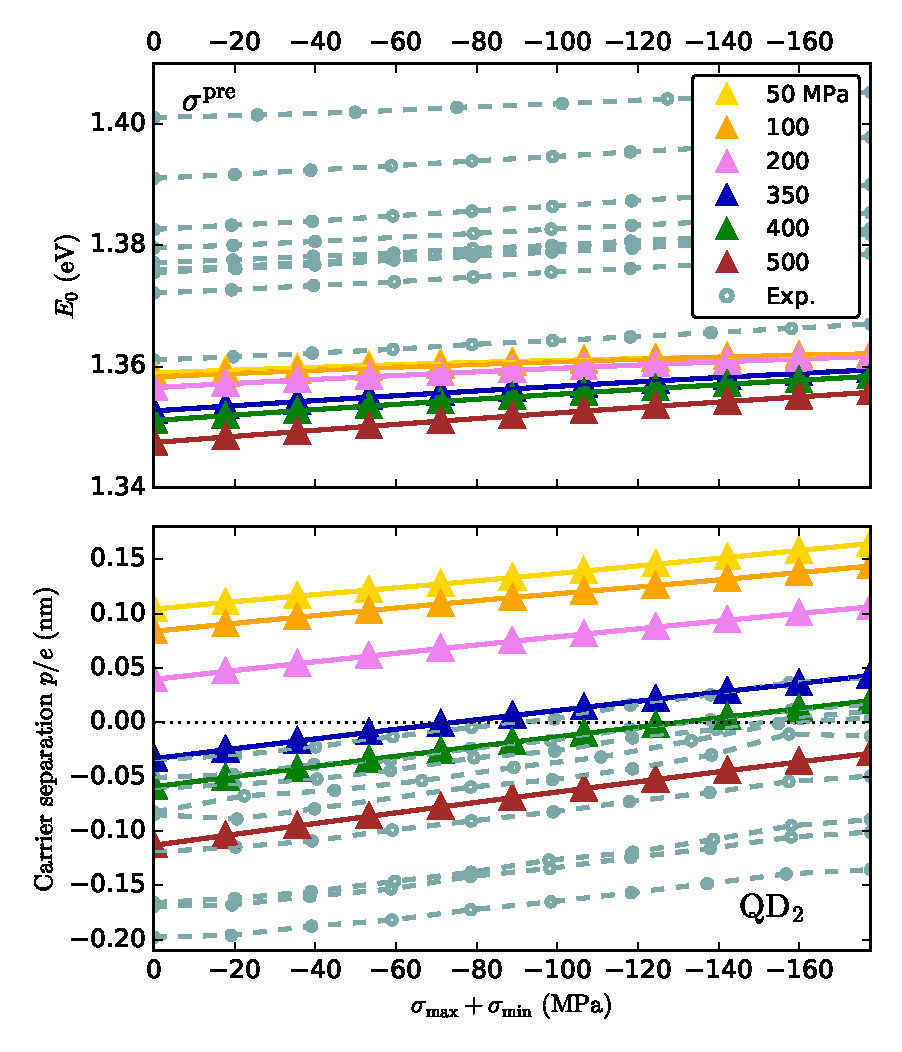
\includegraphics[width=0.5\textwidth]{/2_order/Energy/FINAL__171219_8x8_neotocena_++_nn+_35deg_pres500___prestress} \\
		\end{tabular}
	\end{center}
	\caption{
		Dependencies of $E_0$ (top panel) and $p/e$ (bottom panel) on $\sigma_{\mathrm{max}}+\sigma_{\mathrm{min}}$ experimentally obtained from $\mu$PL measurements of nine InGaAs QDs~\cite{Aberl:17} (dashed curves) and that calculated for different values of $\sigma^{\mathrm{pre}}$. Except of $\sigma^{\mathrm{pre}}$ the simulated QDs had the same properties as QD$_2$. The letter $e$ denotes the elementary charge.
		\label{fig:TuningByPrestress}}
\end{figure}
In Ref.~\cite{Klenovsky_2018_InGaAs_straintuned} was pointed to the role of prestress $\sigma^\mathrm{pre}$ causing from bonding the sample onto the piezo actuator. The bonding quality has been shown to significantly affect FSS measured during strain-tuning, which can be reduce with increasing $\sigma^\mathrm{pre}$. The minimal value 1.15~$\mu$eV of FSS was reached for $\sigma^{\mathrm{pre}}=50$~MPa.




In bottom panel of Fig.~\ref{fig:TuningByPrestress} we show $p/e$ for different values of $\sigma^{\mathrm{pre}}$ acting on QD$_2$. The values of $b$ from fit $p/e$ on ${\sigma_{\mathrm{max}}+\sigma_{\mathrm{min}}}$ by linear model~(\ref{eq:strain_model}) decrease with increasing $\sigma^\text{pre}$. Interestingly, $p/e$ attains positive values for  $\sigma^\text{pre}\lesssim 200$~MPa. However, larger values of $\sigma^\text{pre}$ lead to negative values of $p/e$ for $\sigma_{\mathrm{max}}+\sigma_{\mathrm{min}}=0$. 

While $\sigma^{\mathrm{pre}}$ considerably influences the overall magnitude of $p$ it only mildly affects the slope $A^{\mathrm{QD}}$ or the values of $E_0$.
%
%
%

\begin{figure}[!ht]
	\renewcommand{\tabcolsep}{2pt}
	\begin{center}
		\begin{tabular}{c}
			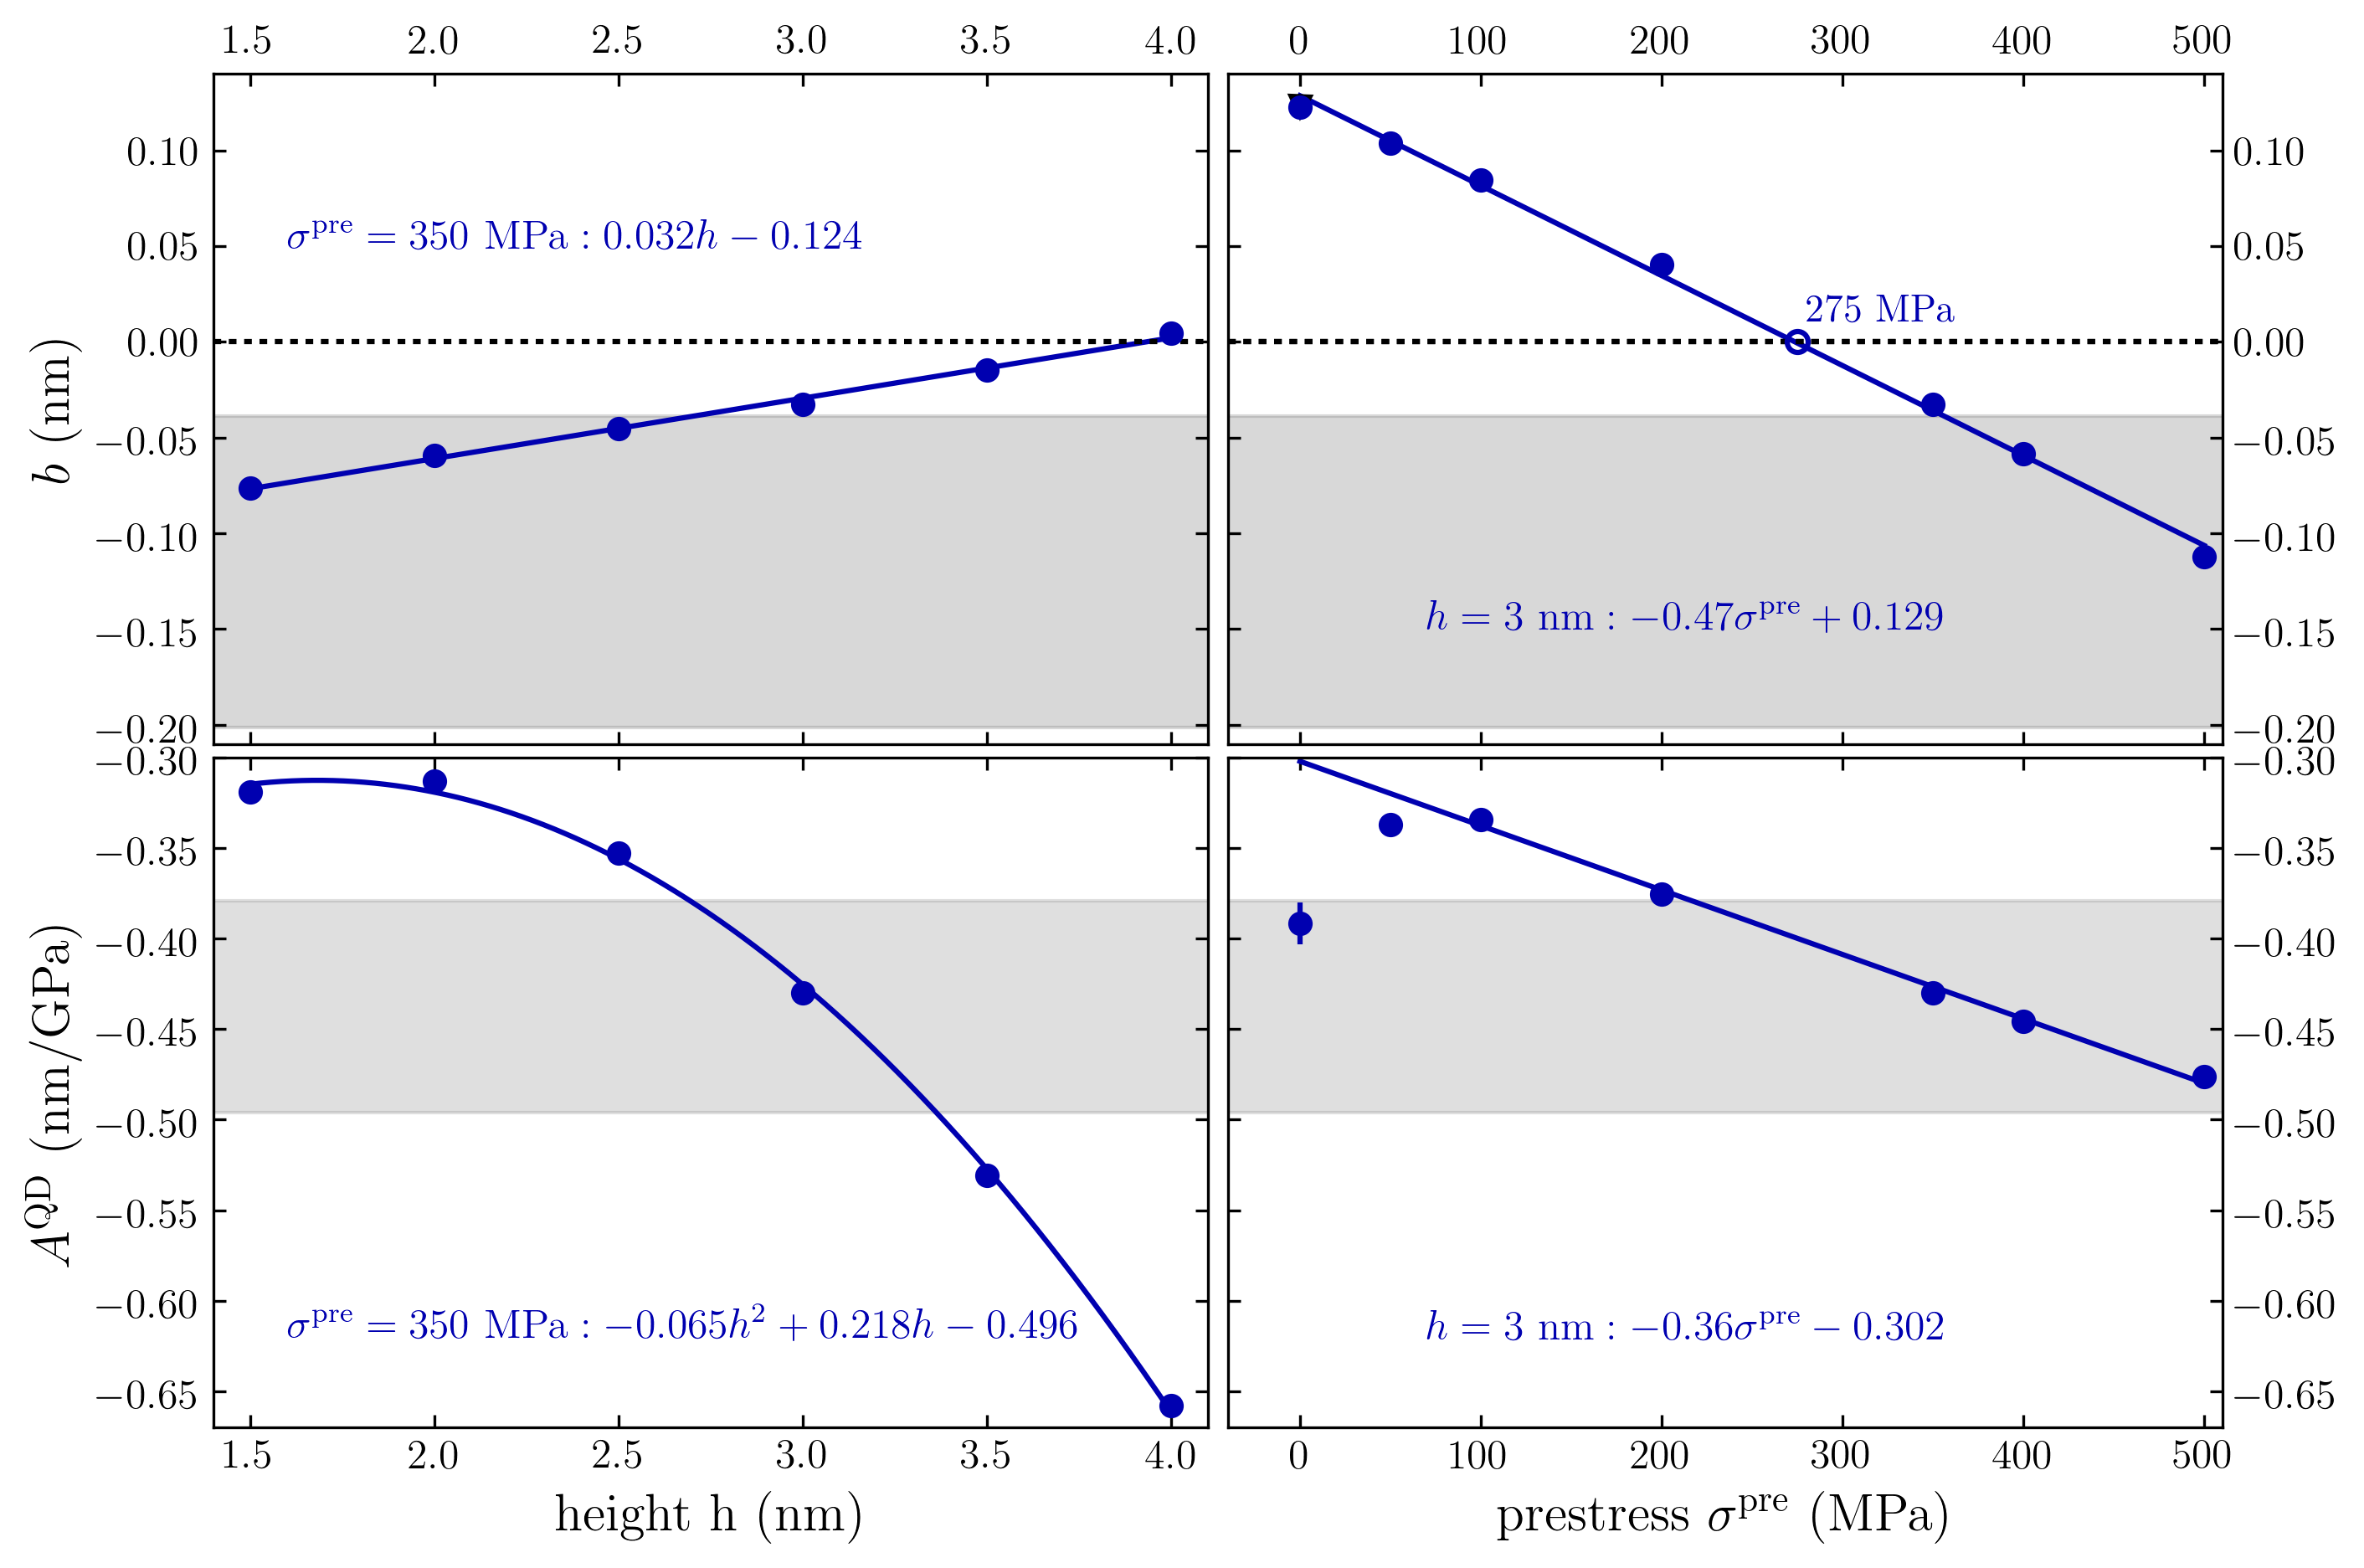
\includegraphics[width=0.9\textwidth]{/2_order/Height_Prestres_fit_pars_3} \\
		\end{tabular}
	\end{center}
	\caption{Evolutions of parameters $A^{\mathrm{QD}}$ and $b$ obtained using linear fit $p/e$ on $\sigma_{\mathrm{max}}+\sigma_{\mathrm{min}}$ for varying (a) height of QD and (b) applied $\sigma^{\mathrm{pre}}$. Full marks represent values received from $\mathbf{k\cdot p}$ calculations, solid lines are fit of the values, empty symbols point to critical values where to $p$ inversion is occurred. The grey shaded area indicate interval of value coming from $\mu$PL measurements.
		\label{fig:FitHeightPrestress}}
\end{figure}
%
For a more detailed analysis of $A^{\mathrm{QD}}$ and $b$ parameters we plot each of the parameter as a function of $\sigma^{\mathrm{pre}}$ and fit them by the linearly increasing behaviour [see Fig.~\ref{fig:FitHeightPrestress}~(b)], the fitted values of the linear model are added in Appendix~\ref{app:empirical_model} in Tab.~\ref{tab:prestress_fit}.

The parameter $b$ can be express as sum of two contributions
\begin{eqnarray}
 b =\frac{1}{e} \left(p^\mathrm{QD} + p^\mathrm{pre} \right)=b_1\sigma^\mathrm{pre} +b_0,
\end{eqnarray} 
%
%
where $p^\mathrm{QD}$ is dipole of QD without bonding and applied stress, $p^\mathrm{pre}$ is effect on $p$ of QD created by adding the sample onto the piezo actuator, which is independent on the applied voltage~\cite{Aberl:17}. Because $\sigma^{\mathrm{pre}}$ acts against to applied stress $\sigma_{\mathrm{max}}+\sigma_{\mathrm{min}}$ resulting in a decrease in $b$ with $\sigma^\mathrm{pre}$ increase. A space to separate charge carriers rises with QD height which leads to observe increase of $b_0=e\times p^\mathrm{QD}$ with the height. Interestingly dependencies of $b$ on $\sigma^\mathrm{pre}$ for several QD heights intersect at one point.

%
%
Moreover using this approach we can estimate $\sigma^\mathrm{pre}_\mathrm{c}$ at which the inversion of $p$ for fixed QD occurs (e.~g., for QD$_2$ we found $\sigma^\mathrm{pre}_\mathrm{0}=275$~MPa).

For $A^{\mathrm{QD}}$, we first observe an increase up to $\sigma^\mathrm{pre}_\mathrm{c}$ followed by a similar linear decrease as for~$b$.

%Similar linear decrease we observe also for $A^{\mathrm{QD}}$ for , .











%








\section{Effect of quantum dot size}

%The emission and dipole moment $p$ of QDs are very sensitive to change not only material composition but also geometrical parameters.
In this section we will focus on tuning $p$ and $E_0$ of QD as well by changing their height, aspect ratio, or diameter.

Firstly, we accomplished calculations for a set of height of QD$_2$ whose results are shown in Fig.~\ref{fig:TuningByHeight}. Emission energies $E_0$ decline with increasing height~\cite{t_schliwa} and can reproduce experimentally obtained $E_0$ in the whole measured range.
%
%
\begin{figure}[ht!]
	\renewcommand{\tabcolsep}{2pt}
	\begin{center}
		\begin{tabular}{c}
			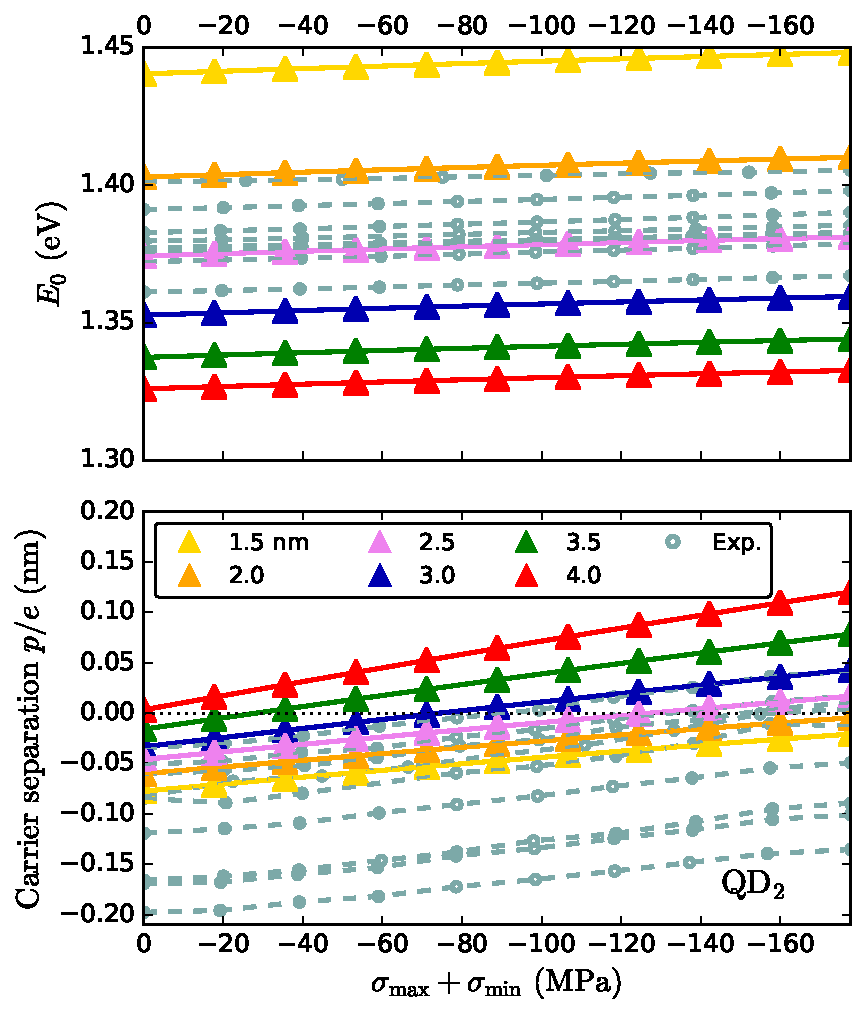
\includegraphics[width=0.5\textwidth]{/2_order/Energy/FINAL__171219_8x8_neotocena_++_nn+_35deg_pres350___40x20_height} \\
		\end{tabular}
	\end{center}
	\caption{
		Dependencies of $E_0$ (top panel) and $p/e$ (bottom panel) on $\sigma_{\mathrm{max}}+\sigma_{\mathrm{min}}$ experimentally obtained from $\mu$PL measurements of nine InGaAs QDs~\cite{Aberl:17} (dashed curves) and that calculated for different values of dot height. Except of height the simulated QDs had the same properties as QD$_2$ including the value of $\sigma^{\mathrm{pre}}=350$~MPa. The letter $e$ denotes the elementary charge.
		\label{fig:TuningByHeight}}
\end{figure}

On the other hand, dot height influences both $A^{\mathrm{QD}}$ and $b$ parameters in dependency $p/e$ on $\sigma_{\mathrm{max}}+\sigma_{\mathrm{min}}$. While $b$ is modified only slightly with height, $A^{\mathrm{QD}}$ changes dramatically.




%
%

%

Lateral changes in QD lead to relative shifts of emission energy and $p$ but neither lateral dimension nor aspect (ratio between top and base radius) of QD entail variation in slopes of both quantity which is demonstrated in Fig.~\ref{fig:TuningByLateral}.

\begin{figure}[!ht]
	\renewcommand{\tabcolsep}{2pt}
	\begin{center}
		\begin{tabular}{cc}
			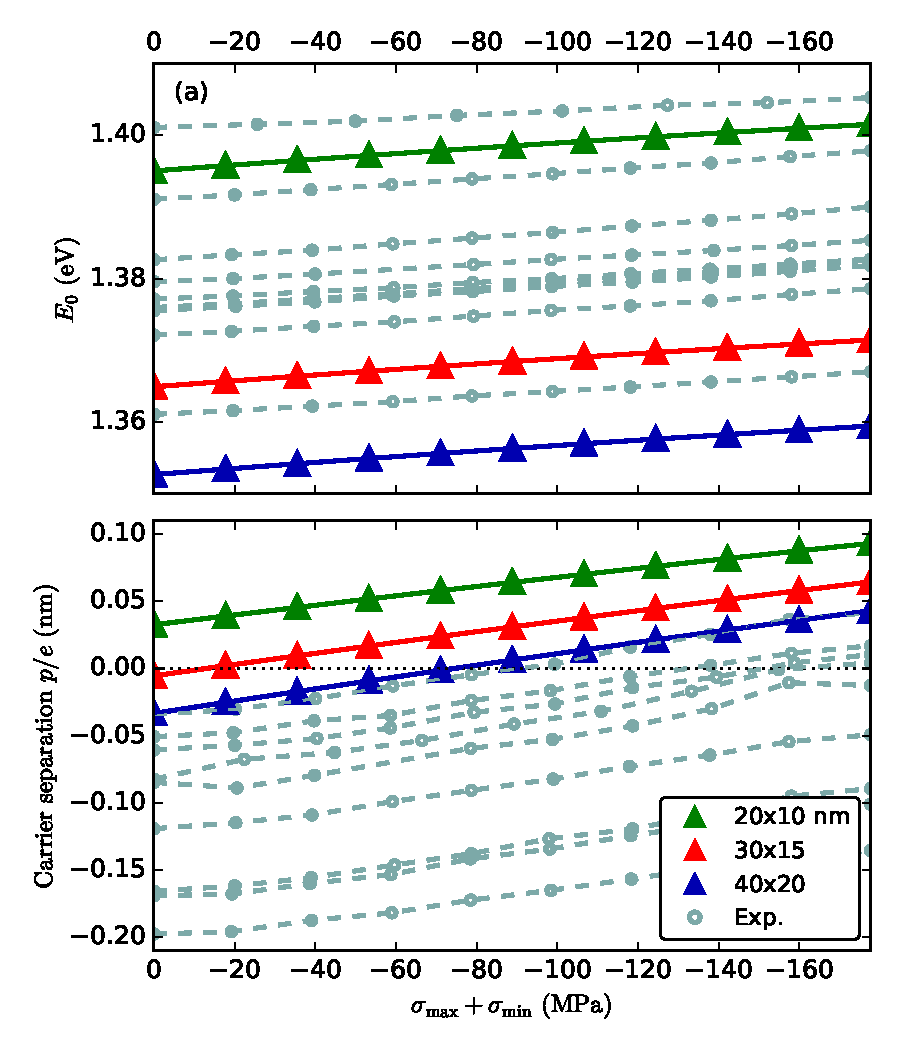
\includegraphics[width=0.5\textwidth]{/2_order/Energy/FINAL__171219_8x8_neotocena_++_nn+_35deg_pres350_h3___lateral} &
			%
			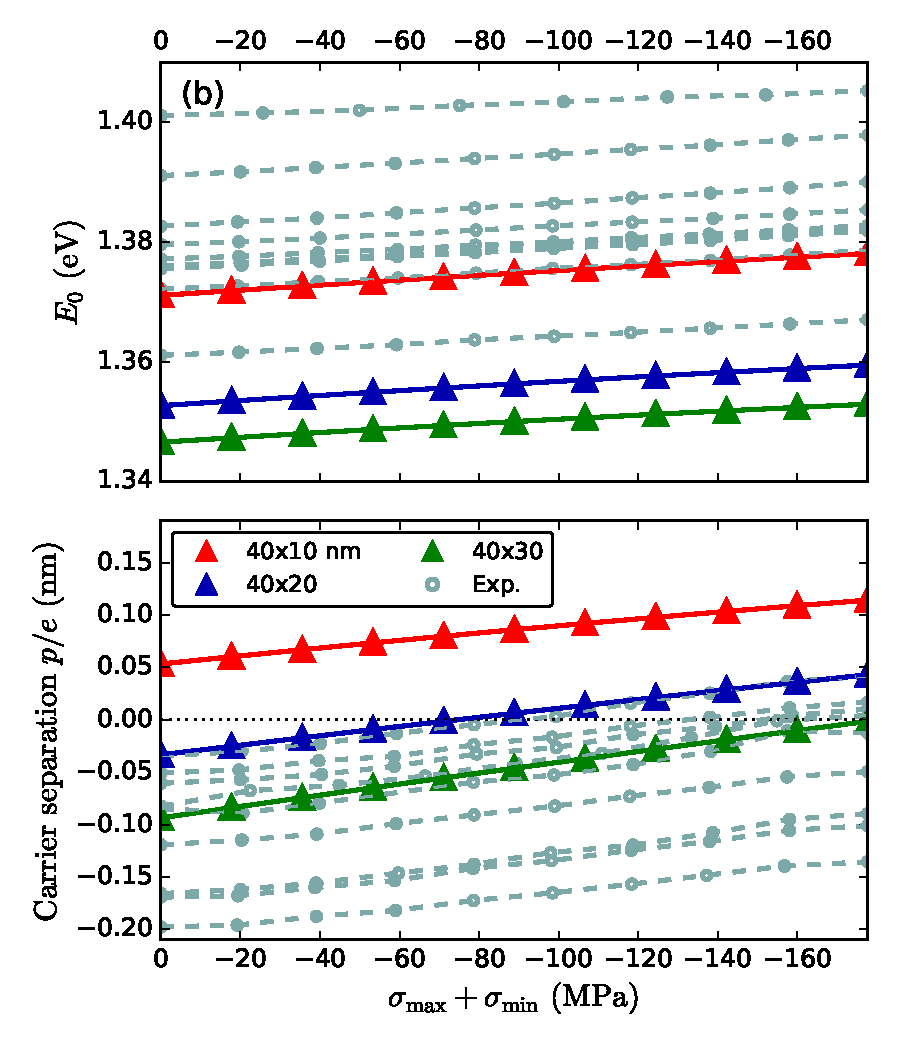
\includegraphics[width=0.5\textwidth]{/2_order/Energy/FINAL__171219_8x8_neotocena_++_nn+_35deg_pres350_h3___aspect} \\
		\end{tabular}
	\end{center}
	\caption{
		Dependencies of $E_0$ (top panels) and $p/e$ (bottom panels) on $\sigma_{\mathrm{max}}+\sigma_{\mathrm{min}}$ experimentally obtained from $\mu$PL measurements of nine InGaAs QDs~\cite{Aberl:17} (dashed curves) and that calculated for different values of (a) dot base diameter with preservation of aspect of 1/2 and (b) aspect with fixed base diameter on 40~nm. Except of various quantity the simulated QDs had the same properties as QD$_2$ including the value of $\sigma^{\mathrm{pre}}=350$~MPa. The letter $e$ denotes the elementary charge.
		\label{fig:TuningByLateral}}
\end{figure}

Because previous analysis have led us to realize that only $\sigma^\mathrm{pre}$ and height are essential for $p$ tuning we repeat processing procedure similar as in precedent, i.e. plot $A^\mathrm{QD}$ and $b$ as a function of height.


We can see in Fig.~\ref{fig:FitHeightPrestress} that both $A^\mathrm{QD}$ and $b$ quadratically evolve with dot height. While $A^\mathrm{QD}$ has monotonic behaviour with $\sigma^\mathrm{pre}$, a character of $b$ is changing from increasing behaviour for small $\sigma^\mathrm{pre}$ (smaller than 500~MPa for our QD$_2$) to falling for large values of $\sigma^\mathrm{pre}$.



%










\newpage

\section{Conclusions}
We have studied the effects of non-linear piezoelectricity on emission energy and electric dipole moment in InGaAs/GaAs quantum dots and pinpointed the importance of that for studies of those systems as compared to using first-order terms only and pinpointed the dominant piezoelectric term. Also, we have elucidated the necessity of the presence of a large built-in in-plane stress due to the lattice mismatch in order for the pronounced changes of the electron-hole dipole due externally applied stress to occur. 

Furthermore, we have illustrated effective way to tune electric dipole moment in quantum dots based on optimization of height of quantum dot and build-in pre-stress. For these quantities we found evolution of parameters from linear fits of the dipole on applied stress. 

Finally in Tab.~\ref{tab:conclusion_straintuned}, we summarize effects of selected parameters on emission energy and electric dipole.

\begin{table*}[ht!]
	\begin{center}
		\caption{Summarize effects of different parameters to tune emission energy $E_0$ and electric dipole $p$ on the hydrostatic applied stress $\sigma^{\rm{app}}=\sigma_{\mathrm{max}}+\sigma_{\mathrm{min}}$ in strain-tuned InGaAs QDs assuming second-order piezoelectricity.  \label{tab:conclusion_straintuned} 
		}
		\begin{tabular}{c|cc|cc}
			\hline \hline
			\multirow{2}{*}{Dependency} &  \multicolumn{2}{c|}{Energy} & \multicolumn{2}{c}{Dipole}\\ \cline{2-5}
			 &   $E_0$ & $\partial E_0/\partial\sigma_\mathrm{app}$  & $b$ & $A^{\mathrm{QD}}$\\  \hline
			 %
			 %
			 %2$^\mathrm{nd}$ piezo&   o & $\textcolor{ps_green}{\boldsymbol{+}}$  & o&$\textcolor{red}{\boldsymbol{-}}$\\ \hline
			 %
			  In contribution &  mean & o  & mean &o\\ \hline
			 %
			 $\sigma^\mathrm{pre}$ &  o &  $\textcolor{ps_green}{\boldsymbol{+}}$  & $\textcolor{red}{\boldsymbol{--}}$ &$\textcolor{red}{\boldsymbol{-}}$\\ \hline
			 %
			 Height&  $\textcolor{ps_green}{\boldsymbol{++}}$&  o  & $\textcolor{ps_green}{\boldsymbol{+}}$ &$\textcolor{ps_green}{\boldsymbol{++}}$\\ \hline
			 %
			 Base &  $\textcolor{ps_green}{\boldsymbol{++}}$&  o   &$\textcolor{ps_green}{\boldsymbol{++}}$ & o\\ \hline
			 %
			 Aspect &  $\textcolor{ps_green}{\boldsymbol{++}}$&  o   &$\textcolor{ps_green}{\boldsymbol{++}}$ & o\\ \hline
			 %
			 %
			 %
			 \multicolumn{5}{c}{o no effect \qquad $\textcolor{ps_green}{\boldsymbol{+}}$ increase \qquad $\textcolor{red}{\boldsymbol{-}}$ decrease }\\
			\hline \hline
		\end{tabular}
	\end{center}
\end{table*}


